\documentclass{SKP-beamer}
\usetikzlibrary{positioning,shapes.geometric}

% NIDS minor project presentation. Replace the four identity fields below.
\title[Network Intrusion Detection System]{Network Intrusion Detection System}
\subtitle{Rule-Based Network Monitoring and Alerting}
\author[Student Name]{Amaresh Sahoo \\
		\small Roll No: 23btics02 \\
                    \small{under the supervision of} \\
                    Asst. Prof. Swetangi Somyadarshi Pati}
\institute[SUIIT]{
                  Department of Computer Science and Engineering \\
                  Sambalpur University Institute of Information Technology \\
                  Jyoti Vihar, Burla, Odisha, India}
\date{\today}
\logo{
\includegraphics[scale=0.42]{suiit.jpg}}
\subject{Minor Project Presentation}

\begin{document}

\begin{frame}
  \titlepage
\end{frame}

\begin{frame}{Schedule}
  \tableofcontents
\end{frame}

\section{Introduction}
\begin{frame}{Why a Network Intrusion Detection System?}
\begin{columns}[T]
\begin{column}{0.57\textwidth}
\begin{block}{Need}
Network activity can include scans, floods, repeated connection attempts, and malicious payloads. Operators need a way to observe traffic and surface suspicious patterns.
\end{block}
\begin{block}{Project goal}
Build a practical, explainable monitor that captures packets, applies configurable rules, stores alerts, and presents them in a protected dashboard.
\end{block}
\end{column}
\begin{column}{0.38\textwidth}
\begin{alertblock}{Project boundary}
This implementation detects and reports suspicious activity. Automated blocking and machine-learning detection are planned extensions, not current features.
\end{alertblock}
\end{column}
\end{columns}
\end{frame}

\begin{frame}{Objectives and Scope}
\begin{block}{Implemented objectives}
\begin{itemize}
  \item Capture live packets and extract network metadata.
  \item Detect selected threats with rule-based checks.
  \item Persist traffic and alerts in SQLite.
  \item Provide authenticated views, filtering, statistics, and report export.
\end{itemize}
\end{block}
\begin{exampleblock}{Out of scope for this version}
Machine-learning classification, automatic firewall changes, and high-throughput production deployment.
\end{exampleblock}
\end{frame}

\section{System Design}
\begin{frame}{System Architecture}
\centering
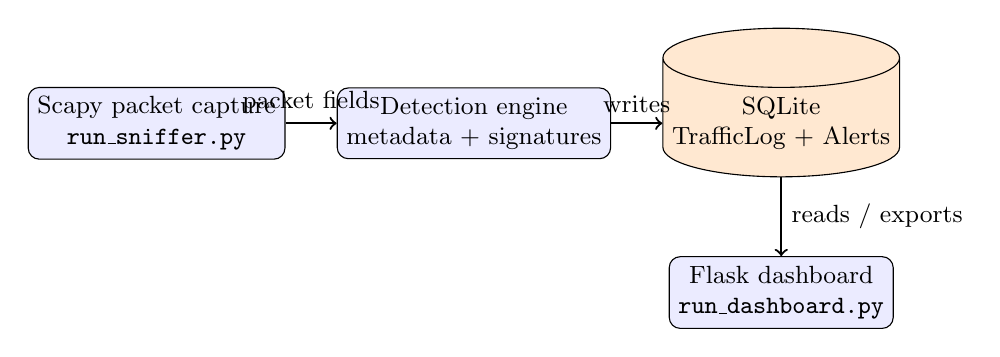
\begin{tikzpicture}[node distance=0.65cm, every node/.style={font=\small},
  box/.style={draw, rounded corners, align=center, minimum width=2.6cm, minimum height=0.8cm, fill=blue!8},
  store/.style={draw, cylinder, shape border rotate=90, aspect=0.25, align=center, minimum width=2.4cm, minimum height=0.9cm, fill=orange!18},
  arr/.style={->, thick}]
  \node[box] (capture) {Scapy packet capture\\\texttt{run\_sniffer.py}};
  \node[box, right=of capture] (detect) {Detection engine\\metadata + signatures};
  \node[store, right=of detect] (db) {SQLite\\TrafficLog + Alerts};
  \node[box, below=1.0cm of db] (web) {Flask dashboard\\\texttt{run\_dashboard.py}};
  \draw[arr] (capture) -- node[above]{packet fields} (detect);
  \draw[arr] (detect) -- node[above]{writes} (db);
  \draw[arr] (db) -- node[right]{reads / exports} (web);
\end{tikzpicture}
\vspace{0.5cm}
\begin{block}{Process separation}
Capture and dashboard run independently and share the database. The blocking capture loop stays outside the web server; SQLite WAL mode supports concurrent reads and writes.
\end{block}
\end{frame}

\begin{frame}{Packet Capture and Data Handling}
\begin{columns}[T]
\begin{column}{0.49\textwidth}
\begin{block}{Captured fields}
Timestamp, source and destination IP, ports, protocol, and packet size are extracted and logged.
\end{block}
\begin{block}{Storage}
SQLite stores traffic records and alert records. WAL mode is enabled for concurrent access by the sniffer and dashboard.
\end{block}
\end{column}
\begin{column}{0.47\textwidth}
\begin{alertblock}{Payload handling}
Payload bytes are inspected in memory for signature matches. Raw payloads are not written to the traffic log; only resulting alerts are persisted.
\end{alertblock}
\begin{exampleblock}{Trusted hosts}
Whitelisted source IPs are skipped before detection rules run.
\end{exampleblock}
\end{column}
\end{columns}
\end{frame}

\section{Detection and Alerts}
\begin{frame}{Rule-Based Detection}
\begin{block}{Implemented checks}
\begin{itemize}
  \item \textbf{Blacklist:} source or destination IP matches a configured list.
  \item \textbf{Port scan:} one source contacts many destination ports in a time window.
  \item \textbf{ICMP flood:} high ICMP packet volume from one source.
  \item \textbf{Repeated connections:} repeated attempts to the same destination and port.
  \item \textbf{Payload signatures:} known SQL injection, XSS, traversal, and EICAR test patterns.
\end{itemize}
\end{block}
\begin{exampleblock}{Explainable decisions}
Each alert is associated with the rule that matched, making the detection path straightforward to inspect and test.
\end{exampleblock}
\end{frame}

\begin{frame}{Alert Pipeline}
\centering
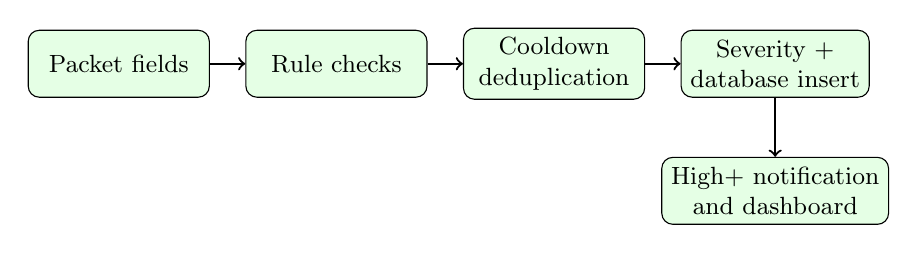
\begin{tikzpicture}[node distance=0.45cm, every node/.style={font=\small},
  box/.style={draw, rounded corners, align=center, minimum width=2.3cm, minimum height=0.85cm, fill=green!10},
  arr/.style={->, thick}]
  \node[box] (packet) {Packet fields};
  \node[box, right=of packet] (rules) {Rule checks};
  \node[box, right=of rules] (cool) {Cooldown\\deduplication};
  \node[box, right=of cool] (save) {Severity +\\database insert};
  \node[box, below=0.75cm of save] (notify) {High+ notification\\and dashboard};
  \draw[arr] (packet) -- (rules);
  \draw[arr] (rules) -- (cool);
  \draw[arr] (cool) -- (save);
  \draw[arr] (save) -- (notify);
\end{tikzpicture}
\vspace{0.5cm}
\begin{block}{Noise control}
Alerts are assigned Low, Medium, High, or Critical severity. A default 30-second cooldown suppresses repeated alerts of the same type from the same source; console notification is enabled for High and above.
\end{block}
\end{frame}

\section{Dashboard}
\begin{frame}{Monitoring Dashboard}
\begin{columns}[T]
\begin{column}{0.49\textwidth}
\begin{block}{Views}
\begin{itemize}
  \item Live traffic
  \item Alert history
  \item Traffic and alert statistics
\end{itemize}
\end{block}
\begin{block}{Investigation}
Filter traffic and alerts by available fields such as protocol, source IP, severity, and alert type.
\end{block}
\end{column}
\begin{column}{0.47\textwidth}
\begin{exampleblock}{Reports}
Export filtered alert data to CSV or PDF.
\end{exampleblock}
\begin{alertblock}{Access control}
Dashboard routes use session-based login. Credentials and the Flask secret key are supplied through environment configuration; debug mode is off by default.
\end{alertblock}
\end{column}
\end{columns}
\end{frame}

\section{Implementation}
\begin{frame}{Technology and Validation}
\begin{columns}[T]
\begin{column}{0.48\textwidth}
\begin{block}{Technology stack}
\begin{itemize}
  \item Python for capture and detection
  \item Scapy for packet inspection
  \item SQLite for local persistence
  \item Flask for dashboard and APIs
  \item ReportLab for PDF reports
\end{itemize}
\end{block}
\end{column}
\begin{column}{0.48\textwidth}
\begin{block}{Validation approach}
Unit tests cover detection rules and dashboard security. Rule checks can be exercised against fabricated traffic rows without capturing live network packets.
\end{block}
\begin{alertblock}{Operational requirement}
Live packet capture generally requires elevated privileges. Run capture and dashboard as separate processes.
\end{alertblock}
\end{column}
\end{columns}
\end{frame}

\begin{frame}{Limitations and Next Steps}
\begin{block}{Current limitations}
\begin{itemize}
  \item Detection is limited to configured rules and known payload signatures.
  \item Rolling-window rules query SQLite per packet and may become a bottleneck at high packet rates.
  \item There is no automatic prevention or machine-learning prediction in this version.
\end{itemize}
\end{block}
\begin{exampleblock}{Planned extensions}
Flow feature extraction and offline-trained anomaly detection; an opt-in prevention module; and dashboard views for model predictions.
\end{exampleblock}
\end{frame}

\section{References}
\begin{frame}{References}
\small
\begin{thebibliography}{9}
\bibitem{scapy} Scapy Project. \emph{Scapy Documentation}. \url{https://scapy.readthedocs.io/}
\bibitem{flask} Pallets Projects. \emph{Flask Documentation}. \url{https://flask.palletsprojects.com/}
\bibitem{sqlite} SQLite Project. \emph{SQLite Documentation}. \url{https://www.sqlite.org/docs.html}
\end{thebibliography}
\end{frame}

\section*{}
\begin{frame}
  \begin{center}
    \begin{pgfpicture}{0cm}{0cm}{3cm}{3cm}
      \pgfmoveto{\pgfxy(3,0)}
      \pgfcurveto{\pgfxy(2,2.2)}{\pgfxy(1,.5)}{\pgforigin}
      \pgfsetlinewidth{2pt}\pgfstroke
      \pgfmoveto{\pgfxy(0,3)}
      \pgfcurveto{\pgfxy(1,.5)}{\pgfxy(2,2.2)}{\pgfxy(3,3)}
      \pgfstroke
      \pgfputlabelrotated{.35}{\pgfxy(0,0)}{\pgfxy(5,3)}{3pt}{\pgfbox[center,base]{\begin{Huge}Thank You!\end{Huge}}}
    \end{pgfpicture}
  \end{center}
\end{frame}

\end{document}
